\chapter{Some useful formulas of atomic physics}

\section{Relationship between measurement strength and scattering rates}
To avoid using reduced dipole moment elements and other quantities in a wrong unit, we can normalize some quantities in terms of characteristic scattering rates and field intensities.
Here are some basic relationships.

Starting from the saturation parameter,
\begin{align}
S(\Delta ) &\equiv \frac{\Omega^2/2}{\Delta^2+\frac{\Gamma^2}{4}} = \frac{S(0)}{4\Omega^2/\Gamma^2+1} \approx \frac{\Omega^2}{2\Delta^2} \quad (\text{for $\Delta^2\gg \Gamma^2$})\\
S(0) &= \frac{I}{I_{\rm sat}}= \frac{2\Omega^2}{\Gamma^2}\\
I_{\rm sat} &= \frac{\hbar \omega}{\sigma_0} \frac{\Gamma}{2}.\label{eq:Isatsigma0}
\end{align}
Therefore, 
\begin{align}\label{eq:OmegaGamma}
\Omega^2 &= \frac{I}{I_{\rm sat}}\frac{\Gamma^2}{2}.
\end{align}


If we define a characteristic scattering rate as
\begin{align}
\gamma_s &\equiv \frac{\Gamma \Omega^2}{4\Delta_{\rm eff}^2},
\end{align}
then the relationships we have derived above (Eqs.~\ref{eq:OmegaGamma} and~\ref{eq:Isatsigma0}) will lead to
\begin{align}
\gamma_s &= \frac{\Gamma^3}{8\Delta_{\rm eff}^2} \frac{I}{I_{\rm sat}}\\
&= \sigma_0 \frac{\Gamma^2}{4\Delta_{\rm eff}^2}\frac{I}{\hbar \omega}.
\end{align}
This final step matches with the physical definition of $ \gamma_s $ that 
\begin{align}
\gamma_s &\equiv N_e \Gamma =\frac{S(\Delta_{\rm eff})}{2} \Gamma\\
&\equiv \sigma(\Delta_{\rm eff}) \frac{I}{\hbar \omega},
\end{align}
where $ \sigma(\Delta)=\frac{\sigma_0}{1+\frac{4\Delta^2}{\Gamma^2}}\approx \sigma_0 \frac{\Gamma^2}{4\Delta^2} $.

We define $ I=\frac{P}{A_{\rm in}}= \frac{\hbar \omega }{A_{\rm in}} \dot{N}_L $, and then
\begin{align}
\gamma_s &= \frac{\sigma_0 }{A_{\rm in}} \frac{\Gamma^2}{4\Delta_{\rm eff}^2}\dot{N}_L.
\end{align}

In a typical spin-squeezing case, the measurement strength may be given by
\begin{align}
\kappa &= \chi_{\rm eff}^2 \dot{N}_L,
\end{align} 
where $ \chi_{\rm eff}= \frac{\sigma_0}{A_{\rm eff}} \frac{\Gamma}{2\Delta_{\rm eff}} $.
Therefore,
\begin{align}
\kappa &= \frac{\sigma_0^2}{A_{\rm eff}^2} \frac{\Gamma^2}{4 \Delta_{\rm eff}^2} \dot{N}_L 
= \frac{A_{\rm in}\sigma_0}{ A_{\rm eff}^2}\gamma_s.
\end{align}


%As an example of spin-squeezing parameter calculation using the formulas above, we plot in Fig.~\ref{fig:QNDproperty_magic44} the optimal peak spin squeezing parameter (with various atom numbers) and OD-related parameters.
%
%\begin{figure}
%\begin{minipage}{.49\linewidth}
%\centering
%\subfloat[]{\label{fig:xi_optimal_NA1000to5000_omega44}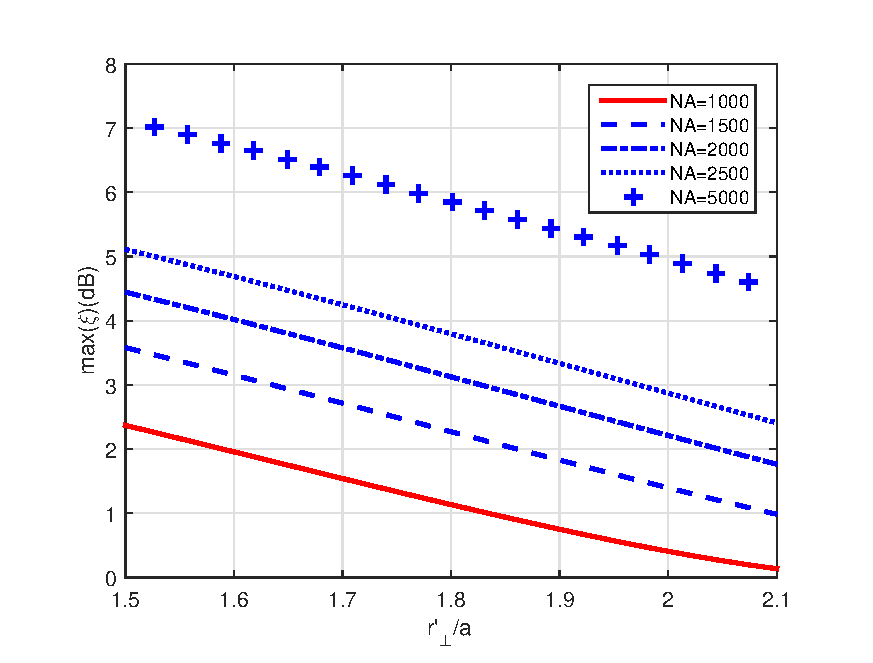
\includegraphics[scale=0.45]{./Figs/xi_optimal_NA1000to5000_omega44}}
%\end{minipage}
%\begin{minipage}{.49\linewidth}
%\centering
%\subfloat[]{\label{fig:OD_optimal_rp}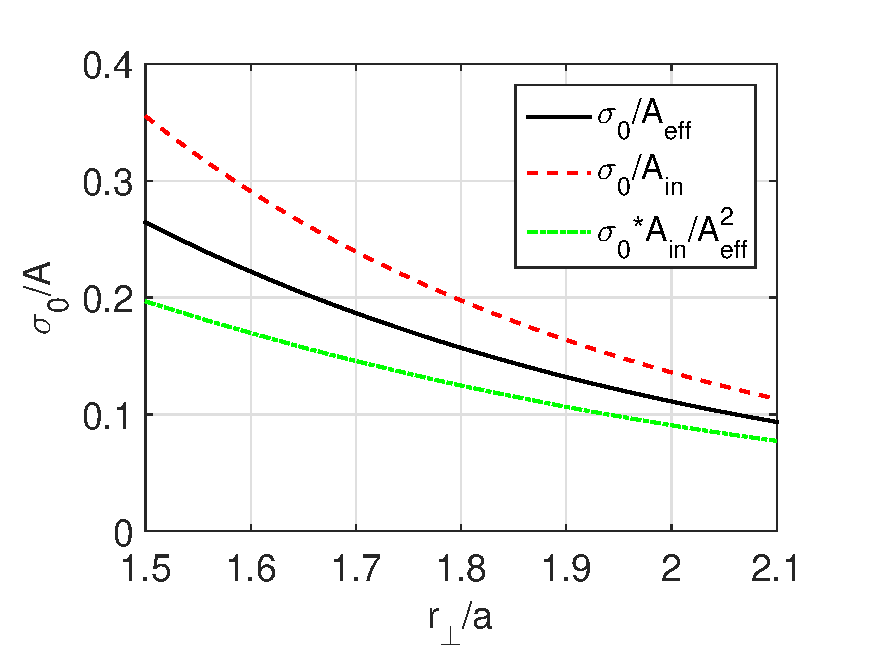
\includegraphics[scale=0.45]{./Figs/OD_optimal_rp}}
%\end{minipage}
%\caption{QND measurement properties using the magic frequency $ \omega_{44} $. Subfigure~\protect\subref{fig:xi_optimal_NA1000to5000_omega44} shows the optimal peak spin squeezing parameter as a function of the radial position of the atom. Different atom numbers have been indicated in different types of lines. Subfigure~\ref{fig:OD_optimal_rp} shows the OD per atom parameters and the ratio of $ \kappa/\gamma_s $ as a function of atoms' radial position when the optimal quantization axis is chosen to plot Subfig.~\protect\subref{fig:xi_optimal_NA1000to5000_omega44}.}\label{fig:QNDproperty_magic44}
%\end{figure}


\section{Relationship between OD/atom and cooperativity}
For atoms prepared in some state, the $\mathrm{OD}/\mathrm{atom}$ can be defined as
\begin{align}
\mathrm{OD}/\mathrm{atom} &= \frac{\sigma_0 }{A_{\rm eff} }, 
\end{align}
where the geometric property of the waveguide or optical medium and the inner structure property of the atoms have been absorbed into the effective mode area factor $ A_{\rm eff} $. 
While in cavity-QED, the concept of cooperativity is usually used to indicate the coupling strength between photons and atoms, and is equivalent to the cavity-to-free-space scattering ratio in the context of atomic cooling~\cite{Tanji-Suzukia2011,Vuletic2000,Kimble1998}. 
In this part, we want to show that the  $\mathrm{OD}/\mathrm{atom}$ in the context of traveling wave and atom interaction has an equivalent definition as the cooperativity in the context of optical cavity QED. 

Below, we consider a two-level atom interacting with an optical mode. 
From Equ.~\ref{Gamma1DGammavac} in the context of nanofiber geometry, we have
\begin{align}
\frac{\Gamma^{1\!D}}{\Gamma} &=   \frac{\sigma_0}{A_{\rm eff}}= \mathrm{OD}/\mathrm{atom}.
\end{align} 
The factor of $ \frac{1}{4} $ has been removed from Equ.~\ref{Gamma1DGammavac} when both propagating directions and polarizations of the modes are summed up in the equation above.

In the context of cavity-QED, the cooperativity per atom is defined as 
\begin{align}
C &= \frac{2 g^2}{\kappa \Gamma},
\end{align}
where $ g=\frac{d\cdot E}{\hbar} $ is the coupling constant between the atom and the cavity mode with reduced dipole momentum $ \mathbf{d}=-e\bra{j}|\br|\ket{j'} $, and $ \kappa  $ and $ \Gamma $ are the decay rates of the cavity and atom respectively. 
One can use the relations that 
\begin{align}
E &= \sqrt{\frac{2\pi\hbar \omega}{V_{\rm eff}}}\\
V_{\rm eff} &= A_{\rm eff} L\\
\kappa &= \frac{c}{2L} \frac{1}{F}\\
\Gamma &= \frac{4}{3}\frac{\omega^3}{c^3} \frac{d^2}{\hbar}
\end{align}
where $ F $ is the cavity finesse.
The cooperativity can be then rewrite as
\begin{align}
C &= \frac{4\pi d^2 \omega}{\hbar A_{\rm eff}L}\cdot  \frac{2L}{c}F \cdot \frac{3}{4} \frac{c^3}{\omega^3} \frac{\hbar}{d^2} = \frac{6\pi c^2}{\omega^2} \frac{1}{A_{\rm eff}} F\\
&= \frac{3\lambda^2}{2\pi} \frac{1}{A_{\rm eff}} F = \frac{\sigma_0}{A_{\rm eff}} F\\
&= \frac{\mathrm{OD}}{\mathrm{atom}} F.
\end{align}

For a Fabry–Pérot type cavity, the finesse is defined as the number of round trip a photon can make before leaking out, which only depends on the mirror reflectivity of the cavity. 
Alternatively, in terms of Q-factor, the finesse of a cavity can be written as $ F= Q\nu_F/\nu_0= Q \pi c/L\omega_0 $ with the Q-factor $ Q=\frac{\nu_0}{\delta\nu} $ and $ \nu_0 $ is the resonant frequency and $ \nu_F $ is the resonant frequency spacing~\cite{Saleh2007}. 
Giving a Gaussian mode with mode waist $ W_0 $, the cooperativity of an atom in the cavity becomes
\begin{align}
C &= \frac{\sigma_0}{\pi W_0^2} F = \frac{\sigma_0}{A} F = \frac{\mathrm{OD}}{\mathrm{atom}} F.
\end{align}
This result agrees with literature~\cite{Hunger2010}. 

To increase the coupling strength between atoms and photons with a nanofiber, the atom number plays the role of cavity finesse in the context of optical cavity and relaxes the requirement of optical mode confinement in the dispersive regime. 